\documentclass[oneside,11pt]{article}
\usepackage{amsmath}
\usepackage{amssymb}
\usepackage{tikz}
\usetikzlibrary{decorations.pathmorphing,arrows}

\begin{document}

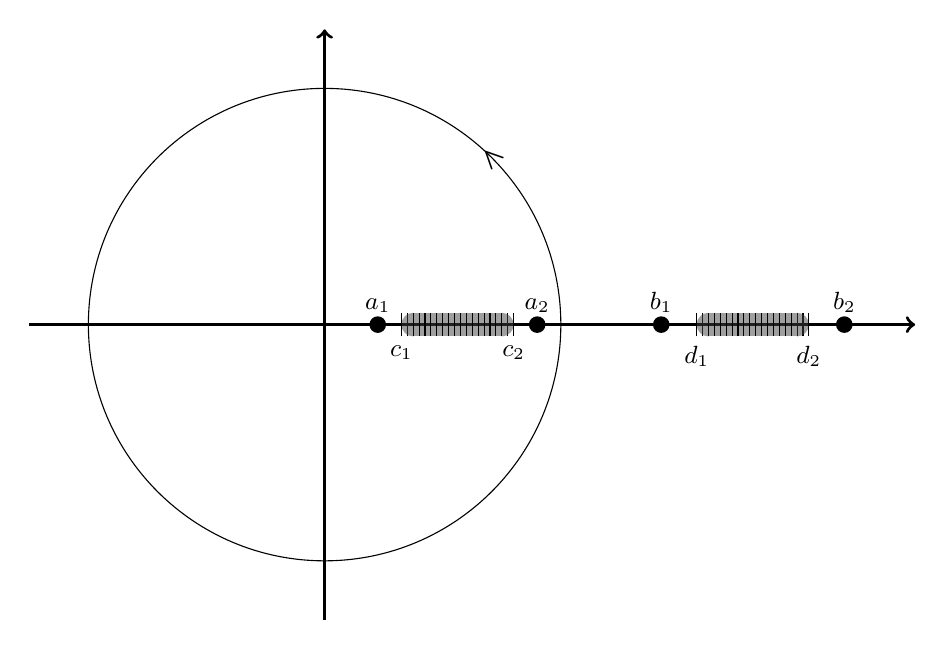
\begin{tikzpicture}[xscale=1.5,yscale=1.5]
	\draw[very thick,->] (-2.5,0) -- (5,0);
	\draw[very thick,->] (0,-2.5) -- (0,2.5);
	\draw[line width=0.3cm, black!75!white, opacity=0.5] (0.75,0) -- (1.5,0);
	\foreach \t in {0.65,0.7,0.75,...,1.6}{
		\draw[thin] (\t,-0.1) -- (\t,0.1);}
	\fill[black!75!white, opacity=0.5] (0.75,0) -- (0.75,0.1) arc (90:270:0.1cm) -- cycle;
	\fill[black!75!white, opacity=0.5] (1.5,0) -- (1.5,0.1) arc (90:-90:0.1cm) -- cycle;
	\draw (0.65,0.1) -- (0.65,-0.1) node[below] {\small $c_1$};
	\draw (1.6,0.1) -- (1.6,-0.1) node[below] {\small $c_2$};
	\draw (0,0) circle (2cm);
	\fill (0.45,0) circle (2pt) node[above=1pt] {\small $a_1$};
	\fill (1.8,0) circle (2pt) node[above=1pt] {\small $a_2$};
	\begin{scope}[xshift=2.5cm]
	\draw[line width=0.3cm, black!75!white, opacity=0.5] (0.75,0) -- (1.5,0);
	\foreach \t in {0.65,0.7,0.75,...,1.6}{
		\draw[thin] (\t,-0.1) -- (\t,0.1);}
	\fill[black!75!white, opacity=0.5] (0.75,0) -- (0.75,0.1) arc (90:270:0.1cm) -- cycle;
	\fill[black!75!white, opacity=0.5] (1.5,0) -- (1.5,0.1) arc (90:-90:0.1cm) -- cycle;
	\draw (0.65,0.1) -- (0.65,-0.1) node[below] {\small $d_1$};
	\draw (1.6,0.1) -- (1.6,-0.1) node[below] {\small $d_2$};
	\fill (0.35,0) circle (2pt) node[above=1pt] {\small $b_1$};
	\fill (1.9,0) circle (2pt) node[above=1pt] {\small $b_2$};
	\end{scope}
	\draw (45:2cm) node[rotate=135] {\small $\boldsymbol{>}$};
\end{tikzpicture}

\end{document}